\documentclass[border=10pt]{standalone}

\usepackage{tikz}
\usepackage{tikzsymbols}
\usetikzlibrary{calc,patterns,shapes.geometric}

\def\centerarc[#1](#2)(#3:#4:#5){\draw[#1] ($(#2)+({#5*cos(#3)},{#5*sin(#3)})$) arc (#3:#4:#5);}

\begin{document}
	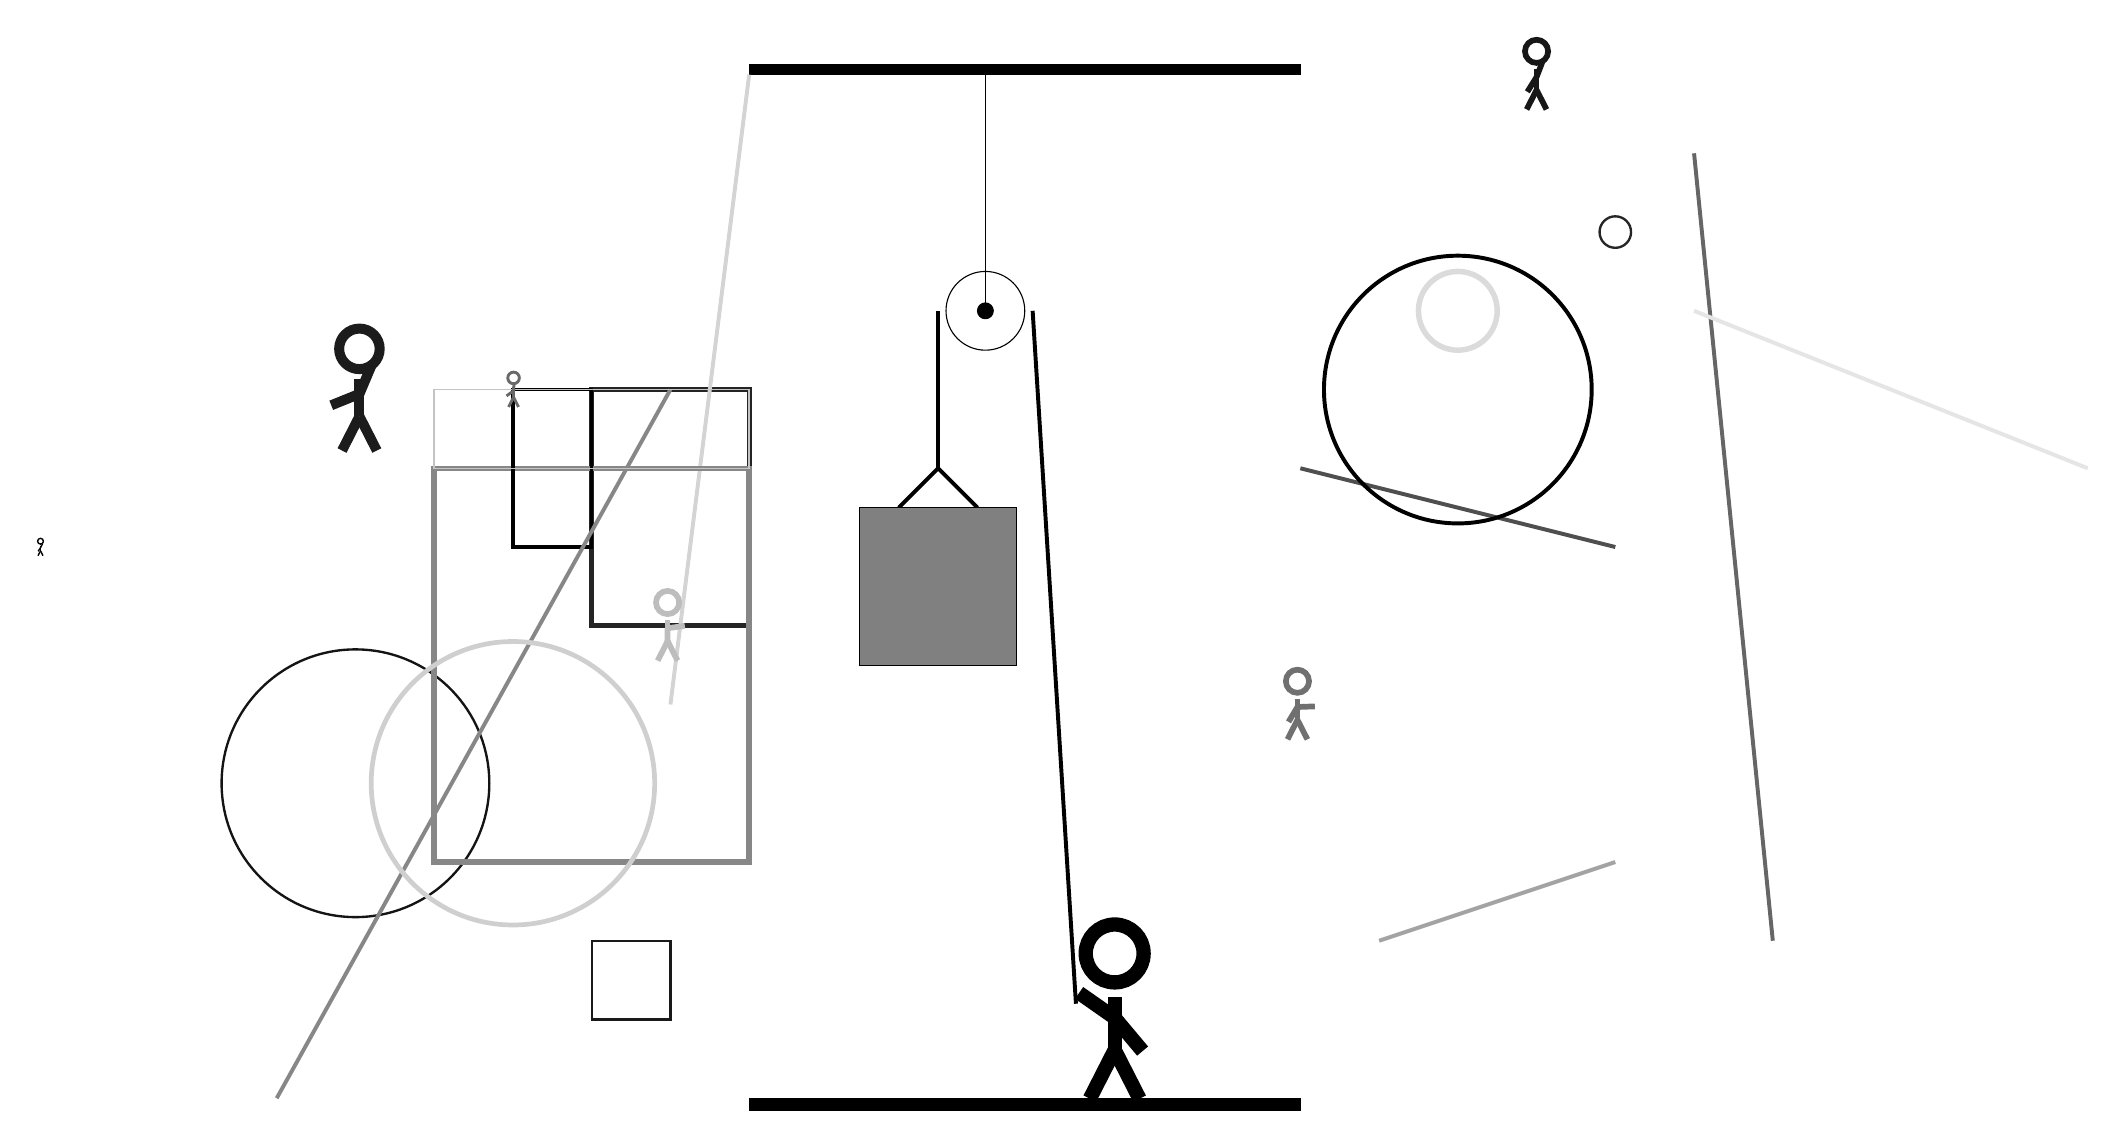
\begin{tikzpicture}
		%%%%% START %%%%%
		
		\draw[fill=black] (-2, 10) rectangle (5, 10.125);
		
		\draw (1, 7) circle (0.5);
		\draw[fill=black] (1, 7) circle (0.1);
		\draw (1, 10) -- (1, 7);
		
		\draw[line width=0.6mm, color=black!86] (-2, 3) rectangle (-4, 6);
		
		\node[line width=0.6mm, color=black!89] at (-7, 6) {\Strichmaxerl[7][22][67]};
		\node[line width=0.6mm, color=black!91] at (8, 10) {\Strichmaxerl[4][58][69]};
		\draw[line width=0.5mm, color=black!17](-2, 10) -- (-3, 2);
		\draw [line width=0.3mm, color=black!92](-7, 1) circle (1.7);
		\draw[line width=0.7mm, color=black!47] (-2, 0) rectangle (-6, 5);
		
		\draw[line width=0.3mm, color=black!90] (-4, -1) rectangle (-3, -2);
		
		\draw[line width=0.4mm, color=black!100] (-4, 4) rectangle (-5, 6);
		\node[line width=0.5mm, color=black!56] at (5, 2) {\Strichmaxerl[4][59][2]};
		\draw[line width=0.5mm, color=black!60](10, 9) -- (11, -1);
		\node[line width=0.2mm, color=black!97] at (-11, 4) {\Strichmaxerl[1][57][62]};
		\node[line width=0.2mm, color=black!26] at (-3, 3) {\Strichmaxerl[4][89][8]};
		\draw[line width=0.5mm, color=black!47](-3, 6) -- (-8, -3);
		
		\draw[line width=0.5mm, color=black!69](5, 5) -- (9, 4);
		\draw [line width=0.7mm, color=black!14](7, 7) circle (0.5);
		\draw [line width=0.3mm, color=black!85](9, 8) circle (0.2);
		\draw[line width=0.2mm, color=black!23] (-2, 5) rectangle (-6, 6);
		
		\node[line width=0.2mm, color=black!59] at (-5, 6) {\Strichmaxerl[2][36][86]};
		\draw [line width=0.6mm, color=black!19](-5, 1) circle (1.8);
		\draw[line width=0.5mm, color=black!36](6, -1) -- (9, 0);
		\draw [line width=0.5mm, color=black!100](7, 6) circle (1.7);
		
		\draw[line width=0.5mm, color=black!10](10, 7) -- (15, 5);
		
		\draw[line width=0.5mm] (-0.1, 4.5) -- (0.4, 5.0) -- (0.9, 4.5);
		\draw[fill=black!50] (-0.6, 4.5) rectangle (1.4, 2.5);
		
		\draw[line width=0.5mm] (0.4, 7) -- (0.4, 5.0);
		\centerarc[line width=0.5mm](1, 7)(0:180:0.6);
		\draw[line width=0.5mm](1.6, 7) -- (2.15, -1.8);
		
		\node at (2.6, -1.9) {\Strichmaxerl[10][-35][-50]};
		
		\draw[fill=black] (-2, -3) rectangle (5, -3.15);
		
		%%%%% END %%%%%
	\end{tikzpicture}
\end{document}